%% bare_conf.tex
%% V1.3
%% 2007/01/11
%% by Michael Shell
%% See:
%% http://www.michaelshell.org/
%% for current contact information.
%%
%% This is a skeleton file demonstrating the use of IEEEtran.cls
%% (requires IEEEtran.cls version 1.7 or later) with an IEEE conference paper.
%%
%% Support sites:
%% http://www.michaelshell.org/tex/ieeetran/
%% http://www.ctan.org/tex-archive/macros/latex/contrib/IEEEtran/
%% and
%% http://www.ieee.org/

%%*************************************************************************
%% Legal Notice:
%% This code is offered as-is without any warranty either expressed or
%% implied; without even the implied warranty of MERCHANTABILITY or
%% FITNESS FOR A PARTICULAR PURPOSE! 
%% User assumes all risk.
%% In no event shall IEEE or any contributor to this code be liable for
%% any damages or losses, including, but not limited to, incidental,
%% consequential, or any other damages, resulting from the use or misuse
%% of any information contained here.
%%
%% All comments are the opinions of their respective authors and are not
%% necessarily endorsed by the IEEE.
%%
%% This work is distributed under the LaTeX Project Public License (LPPL)
%% ( http://www.latex-project.org/ ) version 1.3, and may be freely used,
%% distributed and modified. A copy of the LPPL, version 1.3, is included
%% in the base LaTeX documentation of all distributions of LaTeX released
%% 2003/12/01 or later.
%% Retain all contribution notices and credits.
%% ** Modified files should be clearly indicated as such, including  **
%% ** renaming them and changing author support contact information. **
%%
%% File list of work: IEEEtran.cls, IEEEtran_HOWTO.pdf, bare_adv.tex,
%%                    bare_conf.tex, bare_jrnl.tex, bare_jrnl_compsoc.tex
%%*************************************************************************

% *** Authors should verify (and, if needed, correct) their LaTeX system  ***
% *** with the testflow diagnostic prior to trusting their LaTeX platform ***
% *** with production work. IEEE's font choices can trigger bugs that do  ***
% *** not appear when using other class files.                            ***
% The testflow support page is at:
% http://www.michaelshell.org/tex/testflow/



% Note that the a4paper option is mainly intended so that authors in
% countries using A4 can easily print to A4 and see how their papers will
% look in print - the typesetting of the document will not typically be
% affected with changes in paper size (but the bottom and side margins will).
% Use the testflow package mentioned above to verify correct handling of
% both paper sizes by the user's LaTeX system.
%
% Also note that the "draftcls" or "draftclsnofoot", not "draft", option
% should be used if it is desired that the figures are to be displayed in
% draft mode.
%
\documentclass[10pt, conference, compsocconf]{IEEEtran}
% Add the compsocconf option for Computer Society conferences.
%
% If IEEEtran.cls has not been installed into the LaTeX system files,
% manually specify the path to it like:
% \documentclass[conference]{../sty/IEEEtran}





% Some very useful LaTeX packages include:
% (uncomment the ones you want to load)


% *** MISC UTILITY PACKAGES ***
%
%\usepackage{ifpdf}
% Heiko Oberdiek's ifpdf.sty is very useful if you need conditional
% compilation based on whether the output is pdf or dvi.
% usage:
% \ifpdf
%   % pdf code
% \else
%   % dvi code
% \fi
% The latest version of ifpdf.sty can be obtained from:
% http://www.ctan.org/tex-archive/macros/latex/contrib/oberdiek/
% Also, note that IEEEtran.cls V1.7 and later provides a builtin
% \ifCLASSINFOpdf conditional that works the same way.
% When switching from latex to pdflatex and vice-versa, the compiler may
% have to be run twice to clear warning/error messages.






% *** CITATION PACKAGES ***
%
%\usepackage{cite}
% cite.sty was written by Donald Arseneau
% V1.6 and later of IEEEtran pre-defines the format of the cite.sty package
% \cite{} output to follow that of IEEE. Loading the cite package will
% result in citation numbers being automatically sorted and properly
% "compressed/ranged". e.g., [1], [9], [2], [7], [5], [6] without using
% cite.sty will become [1], [2], [5]--[7], [9] using cite.sty. cite.sty's
% \cite will automatically add leading space, if needed. Use cite.sty's
% noadjust option (cite.sty V3.8 and later) if you want to turn this off.
% cite.sty is already installed on most LaTeX systems. Be sure and use
% version 4.0 (2003-05-27) and later if using hyperref.sty. cite.sty does
% not currently provide for hyperlinked citations.
% The latest version can be obtained at:
% http://www.ctan.org/tex-archive/macros/latex/contrib/cite/
% The documentation is contained in the cite.sty file itself.






% *** GRAPHICS RELATED PACKAGES ***
%
\ifCLASSINFOpdf
   \usepackage[pdftex]{graphicx}
  % declare the path(s) where your graphic files are
  % \graphicspath{{../pdf/}{../jpeg/}}
  % and their extensions so you won't have to specify these with
  % every instance of \includegraphics
  % \DeclareGraphicsExtensions{.pdf,.jpeg,.png}
\else
  % or other class option (dvipsone, dvipdf, if not using dvips). graphicx
  % will default to the driver specified in the system graphics.cfg if no
  % driver is specified.
   \usepackage[dvips]{graphicx}
  % declare the path(s) where your graphic files are
  % \graphicspath{{../eps/}}
  % and their extensions so you won't have to specify these with
  % every instance of \includegraphics
  % \DeclareGraphicsExtensions{.eps}
\fi
% graphicx was written by David Carlisle and Sebastian Rahtz. It is
% required if you want graphics, photos, etc. graphicx.sty is already
% installed on most LaTeX systems. The latest version and documentation can
% be obtained at: 
% http://www.ctan.org/tex-archive/macros/latex/required/graphics/
% Another good source of documentation is "Using Imported Graphics in
% LaTeX2e" by Keith Reckdahl which can be found as epslatex.ps or
% epslatex.pdf at: http://www.ctan.org/tex-archive/info/
%
% latex, and pdflatex in dvi mode, support graphics in encapsulated
% postscript (.eps) format. pdflatex in pdf mode supports graphics
% in .pdf, .jpeg, .png and .mps (metapost) formats. Users should ensure
% that all non-photo figures use a vector format (.eps, .pdf, .mps) and
% not a bitmapped formats (.jpeg, .png). IEEE frowns on bitmapped formats
% which can result in "jaggedy"/blurry rendering of lines and letters as
% well as large increases in file sizes.
%
% You can find documentation about the pdfTeX application at:
% http://www.tug.org/applications/pdftex





% *** MATH PACKAGES ***
%
%\usepackage[cmex10]{amsmath}
% A popular package from the American Mathematical Society that provides
% many useful and powerful commands for dealing with mathematics. If using
% it, be sure to load this package with the cmex10 option to ensure that
% only type 1 fonts will utilized at all point sizes. Without this option,
% it is possible that some math symbols, particularly those within
% footnotes, will be rendered in bitmap form which will result in a
% document that can not be IEEE Xplore compliant!
%
% Also, note that the amsmath package sets \interdisplaylinepenalty to 10000
% thus preventing page breaks from occurring within multiline equations. Use:
%\interdisplaylinepenalty=2500
% after loading amsmath to restore such page breaks as IEEEtran.cls normally
% does. amsmath.sty is already installed on most LaTeX systems. The latest
% version and documentation can be obtained at:
% http://www.ctan.org/tex-archive/macros/latex/required/amslatex/math/





% *** SPECIALIZED LIST PACKAGES ***
%
%\usepackage{algorithmic}
% algorithmic.sty was written by Peter Williams and Rogerio Brito.
% This package provides an algorithmic environment fo describing algorithms.
% You can use the algorithmic environment in-text or within a figure
% environment to provide for a floating algorithm. Do NOT use the algorithm
% floating environment provided by algorithm.sty (by the same authors) or
% algorithm2e.sty (by Christophe Fiorio) as IEEE does not use dedicated
% algorithm float types and packages that provide these will not provide
% correct IEEE style captions. The latest version and documentation of
% algorithmic.sty can be obtained at:
% http://www.ctan.org/tex-archive/macros/latex/contrib/algorithms/
% There is also a support site at:
% http://algorithms.berlios.de/index.html
% Also of interest may be the (relatively newer and more customizable)
% algorithmicx.sty package by Szasz Janos:
% http://www.ctan.org/tex-archive/macros/latex/contrib/algorithmicx/




% *** ALIGNMENT PACKAGES ***
%
%\usepackage{array}
% Frank Mittelbach's and David Carlisle's array.sty patches and improves
% the standard LaTeX2e array and tabular environments to provide better
% appearance and additional user controls. As the default LaTeX2e table
% generation code is lacking to the point of almost being broken with
% respect to the quality of the end results, all users are strongly
% advised to use an enhanced (at the very least that provided by array.sty)
% set of table tools. array.sty is already installed on most systems. The
% latest version and documentation can be obtained at:
% http://www.ctan.org/tex-archive/macros/latex/required/tools/


%\usepackage{mdwmath}
%\usepackage{mdwtab}
% Also highly recommended is Mark Wooding's extremely powerful MDW tools,
% especially mdwmath.sty and mdwtab.sty which are used to format equations
% and tables, respectively. The MDWtools set is already installed on most
% LaTeX systems. The lastest version and documentation is available at:
% http://www.ctan.org/tex-archive/macros/latex/contrib/mdwtools/


% IEEEtran contains the IEEEeqnarray family of commands that can be used to
% generate multiline equations as well as matrices, tables, etc., of high
% quality.


%\usepackage{eqparbox}
% Also of notable interest is Scott Pakin's eqparbox package for creating
% (automatically sized) equal width boxes - aka "natural width parboxes".
% Available at:
% http://www.ctan.org/tex-archive/macros/latex/contrib/eqparbox/

\usepackage{url}



% *** SUBFIGURE PACKAGES ***
%\usepackage[tight,footnotesize]{subfigure}
% subfigure.sty was written by Steven Douglas Cochran. This package makes it
% easy to put subfigures in your figures. e.g., "Figure 1a and 1b". For IEEE
% work, it is a good idea to load it with the tight package option to reduce
% the amount of white space around the subfigures. subfigure.sty is already
% installed on most LaTeX systems. The latest version and documentation can
% be obtained at:
% http://www.ctan.org/tex-archive/obsolete/macros/latex/contrib/subfigure/
% subfigure.sty has been superceeded by subfig.sty.



%\usepackage[caption=false]{caption}
%\usepackage[font=footnotesize]{subfig}
% subfig.sty, also written by Steven Douglas Cochran, is the modern
% replacement for subfigure.sty. However, subfig.sty requires and
% automatically loads Axel Sommerfeldt's caption.sty which will override
% IEEEtran.cls handling of captions and this will result in nonIEEE style
% figure/table captions. To prevent this problem, be sure and preload
% caption.sty with its "caption=false" package option. This is will preserve
% IEEEtran.cls handing of captions. Version 1.3 (2005/06/28) and later 
% (recommended due to many improvements over 1.2) of subfig.sty supports
% the caption=false option directly:
%\usepackage[caption=false,font=footnotesize]{subfig}
%
% The latest version and documentation can be obtained at:
% http://www.ctan.org/tex-archive/macros/latex/contrib/subfig/
% The latest version and documentation of caption.sty can be obtained at:
% http://www.ctan.org/tex-archive/macros/latex/contrib/caption/




% *** FLOAT PACKAGES ***
%
%\usepackage{fixltx2e}
% fixltx2e, the successor to the earlier fix2col.sty, was written by
% Frank Mittelbach and David Carlisle. This package corrects a few problems
% in the LaTeX2e kernel, the most notable of which is that in current
% LaTeX2e releases, the ordering of single and double column floats is not
% guaranteed to be preserved. Thus, an unpatched LaTeX2e can allow a
% single column figure to be placed prior to an earlier double column
% figure. The latest version and documentation can be found at:
% http://www.ctan.org/tex-archive/macros/latex/base/



%\usepackage{stfloats}
% stfloats.sty was written by Sigitas Tolusis. This package gives LaTeX2e
% the ability to do double column floats at the bottom of the page as well
% as the top. (e.g., "\begin{figure*}[!b]" is not normally possible in
% LaTeX2e). It also provides a command:
%\fnbelowfloat
% to enable the placement of footnotes below bottom floats (the standard
% LaTeX2e kernel puts them above bottom floats). This is an invasive package
% which rewrites many portions of the LaTeX2e float routines. It may not work
% with other packages that modify the LaTeX2e float routines. The latest
% version and documentation can be obtained at:
% http://www.ctan.org/tex-archive/macros/latex/contrib/sttools/
% Documentation is contained in the stfloats.sty comments as well as in the
% presfull.pdf file. Do not use the stfloats baselinefloat ability as IEEE
% does not allow \baselineskip to stretch. Authors submitting work to the
% IEEE should note that IEEE rarely uses double column equations and
% that authors should try to avoid such use. Do not be tempted to use the
% cuted.sty or midfloat.sty packages (also by Sigitas Tolusis) as IEEE does
% not format its papers in such ways.





% *** PDF, URL AND HYPERLINK PACKAGES ***
%
%\usepackage{url}
% url.sty was written by Donald Arseneau. It provides better support for
% handling and breaking URLs. url.sty is already installed on most LaTeX
% systems. The latest version can be obtained at:
% http://www.ctan.org/tex-archive/macros/latex/contrib/misc/
% Read the url.sty source comments for usage information. Basically,
% \url{my_url_here}.





% *** Do not adjust lengths that control margins, column widths, etc. ***
% *** Do not use packages that alter fonts (such as pslatex).         ***
% There should be no need to do such things with IEEEtran.cls V1.6 and later.
% (Unless specifically asked to do so by the journal or conference you plan
% to submit to, of course. )


% correct bad hyphenation here
\hyphenation{op-tical net-works semi-conduc-tor}


\begin{document}
%
% paper title
% can use linebreaks \\ within to get better formatting as desired
\title{Usage Management in Cloud Computing}


% author names and affiliations
% use a multiple column layout for up to two different
% affiliations


\author{\IEEEauthorblockN{Pramod A. Jamkhedkar, Christopher C. Lamb, Gregory L. Heileman}
\IEEEauthorblockA{Department of Electrical and Computer Engineering\\
University of New Mexico, Albuquerque, NM 87131-0001 \\
\{pramod54, cclamb, heileman\}@ece.unm.edu}
}


%\author{\IEEEauthorblockN{Authors Name/s per 1st Affiliation (Author)}
%\IEEEauthorblockA{line 1 (of Affiliation): dept. name of organization\\
%line 2: name of organization, acronyms acceptable\\
%line 3: City, Country\\
%line 4: Email: name@xyz.com}
%\and
%\IEEEauthorblockN{Authors Name/s per 2nd Affiliation (Author)}
%\IEEEauthorblockA{line 1 (of Affiliation): dept. name of organization\\
%line 2: name of organization, acronyms acceptable\\
%line 3: City, Country\\
%line 4: Email: name@xyz.com}
%}


% conference papers do not typically use \thanks and this command
% is locked out in conference mode. If really needed, such as for
% the acknowledgment of grants, issue a \IEEEoverridecommandlockouts
% after \documentclass

% for over three affiliations, or if they all won't fit within the width
% of the page, use this alternative format:
% 
%\author{\IEEEauthorblockN{Michael Shell\IEEEauthorrefmark{1},
%Homer Simpson\IEEEauthorrefmark{2},
%James Kirk\IEEEauthorrefmark{3}, 
%Montgomery Scott\IEEEauthorrefmark{3} and
%Eldon Tyrell\IEEEauthorrefmark{4}}
%\IEEEauthorblockA{\IEEEauthorrefmark{1}School of Electrical and Computer Engineering\\
%Georgia Institute of Technology,
%Atlanta, Georgia 30332--0250\\ Email: see http://www.michaelshell.org/contact.html}
%\IEEEauthorblockA{\IEEEauthorrefmark{2}Twentieth Century Fox, Springfield, USA\\
%Email: homer@thesimpsons.com}
%\IEEEauthorblockA{\IEEEauthorrefmark{3}Starfleet Academy, San Francisco, California 96678-2391\\
%Telephone: (800) 555--1212, Fax: (888) 555--1212}
%\IEEEauthorblockA{\IEEEauthorrefmark{4}Tyrell Inc., 123 Replicant Street, Los Angeles, California 90210--4321}}




% use for special paper notices
%\IEEEspecialpapernotice{(Invited Paper)}




% make the title area
\maketitle


\begin{abstract}
User concerns regarding data handling within the cloud will gain increasing importance as cloud computing becomes more pervasive. Existing service level agreement (SLA) frameworks are not designed for flexibly handling  even relatively straightforward usage policies. This paper introduces the notion and importance of usage management in cloud computing. It provides an analysis of features and challenges involved in deploying a usage management framework over a distributed cloud environment to enable automated and actionable interpretation, reasoning and enforcement of usage policies. Finally, a preliminary architecture for such a framework is proposed. 

%In this paper we examine management of cloud-based computing infrastructure, and is related to issues of configuration, data management, security, privacy and regulatory compliance in cloud computing environments. More specifically, the requirements associated with these issues are typically captured in the form of service level agreements (SLAs).  Herein, aspects of developing a comprehensive framework for automating the management of SLAs and acting upon the polices they contain.  We describe a framework that provides usage management services to other cloud computing services for expression, reasoning and validation of policies related to the handling of data and services.  In addition, we will consider how a complicated set of SLAs, corresponding to a set of users and cloud resources, can be evaluated so that feedback can be provided which enables control of the underlying cloud resources in such a way that all of the polices contained in the combined set of SLAs are satisfied. 

\end{abstract}

\begin{IEEEkeywords}
usage management; cloud security; service level agreements; access control

\end{IEEEkeywords}


% For peer review papers, you can put extra information on the cover
% page as needed:
% \ifCLASSOPTIONpeerreview
% \begin{center} \bfseries EDICS Category: 3-BBND \end{center}
% \fi
%
% For peerreview papers, this IEEEtran command inserts a page break and
% creates the second title. It will be ignored for other modes.
\IEEEpeerreviewmaketitle

\section{Introduction}
The characteristics of cloud computing services tend to differ from those of grid and cluster-based computing applications.  Specifically, cloud services tend to be more market oriented, and they typically host entire user applications within the distributed cloud environment. These characteristics raise serious concerns from cloud users' perspective regarding the manner in which their data are handled or used by the cloud services. These metrics are orthogonal to the traditional performance-oriented quality of service (QoS) metrics, and their semantics are well beyond encryption and privacy requirements. Existing service level agreement (SLA) frameworks focus primarily on performance-oriented QoS parameters, and are not designed for expressing and enforcing policies to control the manner and restrictions under which users' data need to be handled~\cite{WSA, WSLA, WSP,PaRaSh:09}. User concerns on data handling in the cloud along with the limitations of existing SLA frameworks to express, reason and enforce data usage policies in an automated manner creates the need for usage management in cloud computing. 
 
Usage management is the collective set of processes and mechanisms that enables one to manage and control how data are
used within a system. This encompasses policy specification languages, licensing mechanisms, policy expression and reasoning mechanisms, policy enforcement mechanisms, usage tracking, along with supporting authentication and encryption mechanisms~\cite{PaSa:04,JaHeLa:10}. The ability to express fine-grained usage policies will provide cloud users with greater trust regarding the usage of their data within clouds, and will provide them with the confidence to employ cloud services. A mechanism to interpret, reason over, and enforce usage policies within clouds in an automated manner will allow cloud providers to optimize resource allocation while ensuring safety and security of cloud users' data. A correct estimation of the cost involved in enforcing usage policies will further enable cloud providers with business opportunities such as yield management and price differentiation. 

This paper introduces the notion of usage management in cloud computing and provides an in-depth analysis of the challenges and principles involved in the design of an open, interoperable usage management framework that operates over a distributed cloud computing environment. The analyses include application of well-known principles of system design and standards~\cite{BlCl:01,Cl:88,ClWrSoBr:02}, research developments in the areas of usage control~\cite{PaSa:04,JaHeLa:10}, policy languages design principles~\cite{JaHeMa:06}, digital rights management (DRM) systems~\cite{JaHe:09},  and interoperability~\cite{JaHe:04,HeJa:05,KoLaMaMi:04} towards the development of such a framework.

The paper delves into how such a framework will improve upon the status quo by leveraging  existing security mechanisms, and enabling automated reasoning of policies with respect to the underlying cloud security infrastructure. Based on these analyses, a system for expressing and reasoning about usage management within a distributed cloud environment is proposed that makes use of a common cloud ontology shared by different cloud services. The proposed system architecture enables usage policies to be expressed in different policy languages, and interpreted across various cloud environments. 

The remainder of the paper is structured as follows. Section~\ref{sec:motivation} introduces the need for incorporating usage management in cloud computing. An analysis of the features of a usage management framework for cloud computing environments is provided in Section~\ref{sec:clouds-usage}. In Section~\ref{sec:architecture} a preliminary architecture for usage management is proposed that makes use of a common cloud ontology and enables use of multiple policy languages. Finally, Section~\ref{sec:conclusions} provides some useful concluding remarks and describes future work. 


% CHRIS-- The manner in which SLAs are currently expressed, interpreted, enforced and monitored has a number of shortcomings that will stifle the development of cloud computing solutions of the future.  A  rudimentary policy option on data security leaves little room for cloud users to express and negotiate their security concerns and requirements. Ideally, the supplier and user of cloud services are able to negotiate the service terms in an agreement that is expressive enough to capture the requirements and concerns of both parties. This requires a user-customizable fine-grained SLA,  as opposed to the current one-size-fits-all model.  We leverage the author's current research and expertise in the areas of usage management and control theory in order to develop a framework that supports usage management in cloud computing.

%CHRIS-- In the following paper, we will first briefly cover current approaches to cloud service management and integration, and demonstrate their shortcomings.  We will then delve into how usage management how a usage management framework would improve the status quo.  We will cover challenges and features of this kind of a system, and existing technologies we must leverage for an acceptable system.  We will close with a description of the architecture of our system and various views into it's structure and operational state.


\section{Motivation and Related Work}\label{sec:motivation}
In the recent years, cloud computing has  managed to emerge as a computing platform that allows computing services to be consumed as a utility by consumers. In cloud computing, applications, systems software, and hardware are offered as utility services to consumers over the Internet. In service-based architectures, service consumers need to be provided with  highly reliable services that meet their expectations. Service consumers indicate these expectations in terms of QoS parameters that are expressed in the form of an SLA negotiated with the service provider. 

In the realm of computing, there exist multiple service-based paradigms such as web-services, cluster computing, grid computing and cloud computing~\cite{Bu:09}. Cloud computing is set apart from the other forms of service-based computing paradigms by a collective set of distinguishing characteristics such as market orientation, virtualization, dynamic provisioning of resources and service composition via multiple service providers~\cite{BuYeVeBrBr:09}. These characteristics imply that in cloud computing,  cloud users' data reside in the cloud for a finite amount of time, that these data are handled by multiple cloud services, and that data fractions may be stored, processed, transformed and routed across a geographically distributed cloud infrastructure. These activities occur ``behind-the-scenes'', within the cloud, while giving cloud users an impression of a single virtual machine.  In current cloud implementations,  cloud users have very little control over the manner in which data are handled by cloud providers, once they are pushed into the cloud. As consumers start aggressively using cloud services, this limitation will become a matter of serious concern. 

The handling or use of cloud users' data within the cloud by different services refers to policies specifying the constraints under which different actions may be carried out on the data. A cloud user may want to limit the manner in which data are stored, routed, or processed, and specify the entities and processes that are authorized to carry out these activities, and under what conditions. As an example, a government agency might want to prevent its data from being stored in one particular country, or prevent routing of the data via a particular set of networks it considers unreliable or insecure. Similarly, a financial company might want to prevent its data from being processed by a particular cloud service, or may want the data to be encrypted before being stored by an untrusted cloud storage service. Usage policies typically consist of a range of semantics such as restrictions on the manner in which data are used, temporal restrictions on usage, spatial or attribute-based restrictions, permissions, obligations, penalties, count-based limits on usage, usage tracking and reporting, and partial dependencies to name a few.   Hence, as cloud services become pervasive, cloud users will want to dictate the terms of usage for their data within the cloud in a manner that is expressive enough to capture their concerns. 


Existing cloud infrastructures and SLA frameworks are ill-equipped to address the requirements and challenges of usage management in distributed cloud systems. At present, cloud providers enable usage management features via rudimentary techniques involving a  one-size-fits-all option, where cloud users have little or no say in expressing usage policies over their data. For example, the Amazon S3 storage service allows a region-based facility where data stored in one region are guaranteed not to leave that particular region~\cite{AWS}. Such options are too coarse and simplistic to address cloud users' concerns. 

Existing service-based computing paradigms such as web services, clusters and grid computing use well-established SLA frameworks that enable expression, interpretation, monitoring, control and enforcement of SLA terms~\cite{WSA, WSLA, WSP,PaRaSh:09}. However, the SLAs supported by these frameworks focus on performance metrics such as availability, reliability, bandwidth, response times, instructions per second, etc. ~\cite{PaSc:06}. Also, the privacy and security metrics supported by these frameworks focus primarily on encryption of data. Performance-based metrics are end-to-end, meaning that users are concerned only with the delivery of performance, and not about the measures taken by service providers to deliver the service. The service provider simply maintains the required quality of service by allocating more resources or employing additional third party services. Compared to this, usage management requirements are different since cloud users potentially have a say in every action taken on their data, throughout the lifetime of the data in the cloud, including scenarios where the data are passed on to a third party provider. 

Usage management requirements are significantly different from QoS-based metrics, and present a new set challenges that are beyond the capabilities of the existing SLA frameworks. It is therefore necessary to design a separate mechanism for usage management that will enable persistent, automated management data usage control, while allowing seamless flow of data in a distributed cloud infrastructure. 



\section{Usage Management in Clouds}\label{sec:clouds-usage}
There exists a rich body of research in the areas of access control~\cite{BlPa:73,BlPa:76}, usage control~\cite{PaSa:04,JaHeLa:10} and DRM~\cite{ArHu:07,HaWe:08, ODRL-req,JaHe:08,XrML-spec}, all of which require usage management.  In this section an analysis of the challenges associated with developing a usage management framework for cloud computing infrastructures is provided. A discussion of how advancements in these areas areas can be leveraged by usage management frameworks is also provided below.

\subsection{Overview}

%In existing cloud systems, the focus of SLAs is on performance based QoS parameters, whereas policies to describe the manner in which user data need to be used are either non-existent, or managed in a primitive way. Figure~\ref{fig:overview} shows a high-level model of the manner in which existing systems implement usage management of user data. The usage management policies are statically defined in an SLA by allowing the user to choose from one of options provided by the cloud provider, such as the Amazon S3 storage region-based options mentioned earlier. The interpretation, enforcement and monitoring of these policies is carried out statically in a hardwired manner by the cloud provider.  Such a static approach for handling usage policies presents numerous problems for usage management discussed below,  that will stifle the full fledged expression of cloud user concerns regarding the correct usage of data. 


Figure~\ref{fig:overview} shows a high-level model of the manner in which existing systems implement usage management of user data. In this setup usage management policies are statically defined in an SLA by allowing cloud users to choose from a set of options provided by the cloud provider. The usage policy monitoring in existing cloud systems, in many instances, is carried out by a person (e.g., a lawyer) as shown in Figure~\ref{fig:overview}.  Such a static approach for handling usage policies presents numerous problems for usage management that stifle full-fledged expression of cloud users' concerns regarding appropriate usage of their data within the cloud.   


\begin{figure}[!t]
\centering
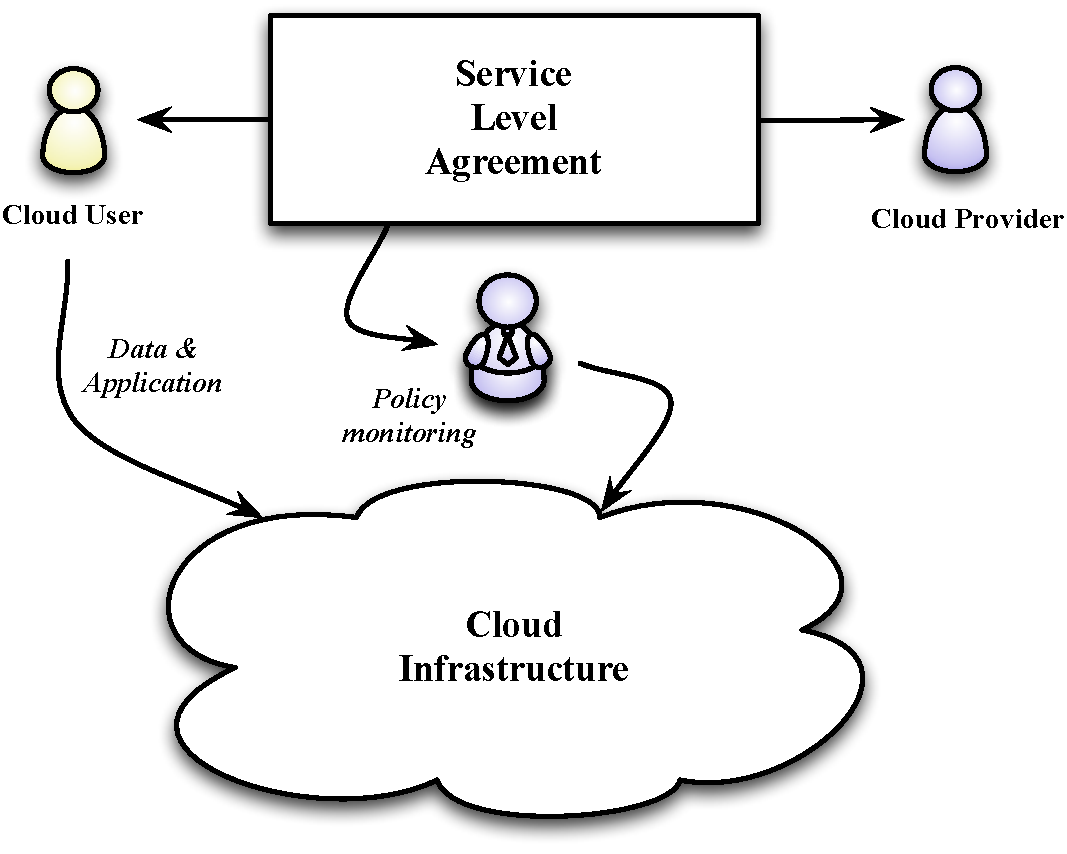
\includegraphics[scale=0.4]{Overview.pdf}
% where an .eps filename suffix will be assumed under latex, 
% and a .pdf suffix will be assumed for pdflatex; or what has been declared
% via \DeclareGraphicsExtensions.
\caption{Usage management in existing cloud environment.}
\label{fig:overview}
\end{figure}

A natural consequence of static or hardwired handling of usage policies is that it prevents incorporation of complex usage policies. In case of solutions that follow the ``one-size-fits-all'' model, users have a limited say or options to express data usage terms. Furthermore, such approaches leaves cloud users with little or no room for negotiation of usage terms with cloud providers. Another major disadvantage of such a static approach is that there does not exist an interconnection between policies and the cloud infrastructure. This means that usage policies are not actionable, and it is not possible to reason about them with respect to the capabilities and limitations of the underlying cloud infrastructure. The lack of reasoning capabilities leads to under-utilization of cloud resources. While this impediment is not a major issue when dealing with simple policies, under-utilization of resources can cause serious revenue loss for cloud providers as the number of users and complexity of policies increase. 



In order to address these concerns, it is necessary that usage policies be managed by means of a usage management framework that will operate over a distributed cloud infrastructure as shown in Figure~\ref{fig:cloud-umf}. In this figure, a  cloud user and a cloud provider negotiate a usage policy and the price associated with the policy in an automated manner via software agents. Existing negotiation frameworks such as the Java Agent Development Framework and the FIPA negotiation protocols can be used for this purpose~\cite{BePoRi:02}.  Next, the policy is represented in a machine-readable and machine-actionable form. A rich body of research in the areas of rights expression languages~\cite{ODRL-req,JaHe:08,XrML-spec}, usage control languages~\cite{PaSa:04,HiPrBaScWa:07}, and access control languages~\cite{BlPa:76}, for formal representation of various usage semantics exists that can be leveraged to this effect. The policy is then interpreted and enforced over a distributed cloud infrastructure making use of existing trusted computing platforms to provide a comprehensive usage management solution. Significant business opportunities become available if these SLAs are easily customizable, allowing for price differentiation and yield management. In order achieve this, a usage management framework operating over a distributed cloud environment needs to be developed that satisfies the following goals:

\begin{enumerate}
\item Fine-grained expression of usage policies that can be negotiated between cloud users and cloud providers. 
\item Seamless movement of data within the cloud and persistent enforcement of usage policies across different services, at all levels of virtualization, along all data transformations throughout the lifetime of data in the cloud. 
\item Actionable policies that enable automated interpretation, reasoning, enforcement, usage tracking and reporting vis-a-vis the underlying cloud infrastructure. 
\end{enumerate}

\begin{figure}[!t]
\centering
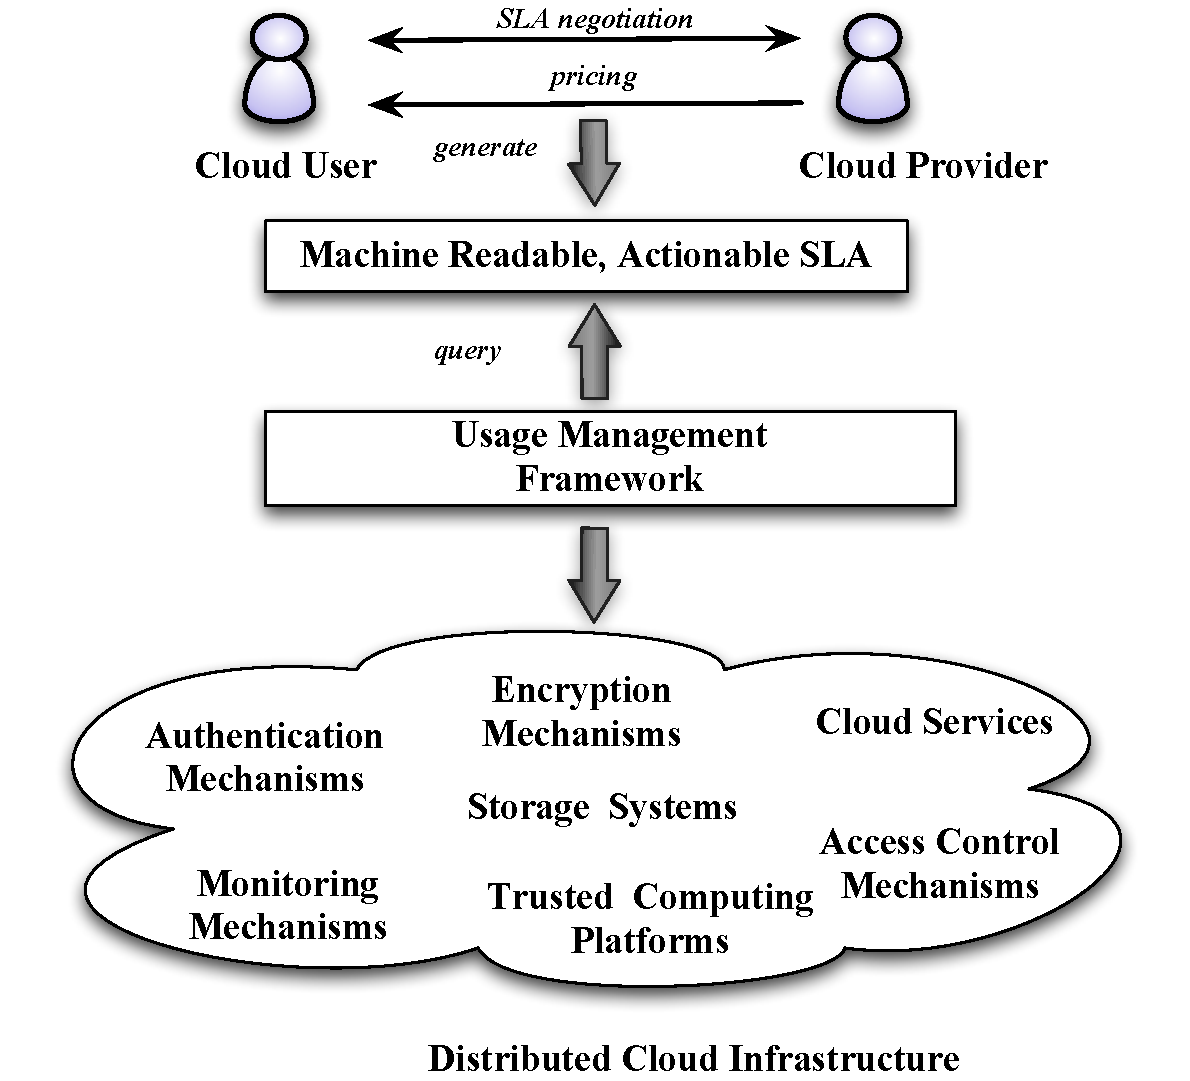
\includegraphics[scale=0.4]{cloud-umf}
% where an .eps filename suffix will be assumed under latex, 
% and a .pdf suffix will be assumed for pdflatex; or what has been declared
% via \DeclareGraphicsExtensions.
\caption{Usage management in cloud.}
\label{fig:cloud-umf}
\end{figure}

The challenges presented by the specifics of a distributed cloud infrastructure in achieving these goals, and the features that such a framework must exhibit in order to address these challenges are discussed next. 

%Explain how the usage management framework must ideally operate as explained in Figure~\ref{fig:cloud-umf}.
%\begin{enumerate}
%\item Fine-grained expression of usage policies negotiable between cloud users and cloud providers.
%\item Consistently operate over a distributed cloud infrastructure at all levels across different services. 
%\item It must be able to interconnect policies with cloud infrastructure to allow interpretation, monitoring, enforcement, and resource allocation. 
%\end{enumerate}

\begin{figure*}[t]
\centering
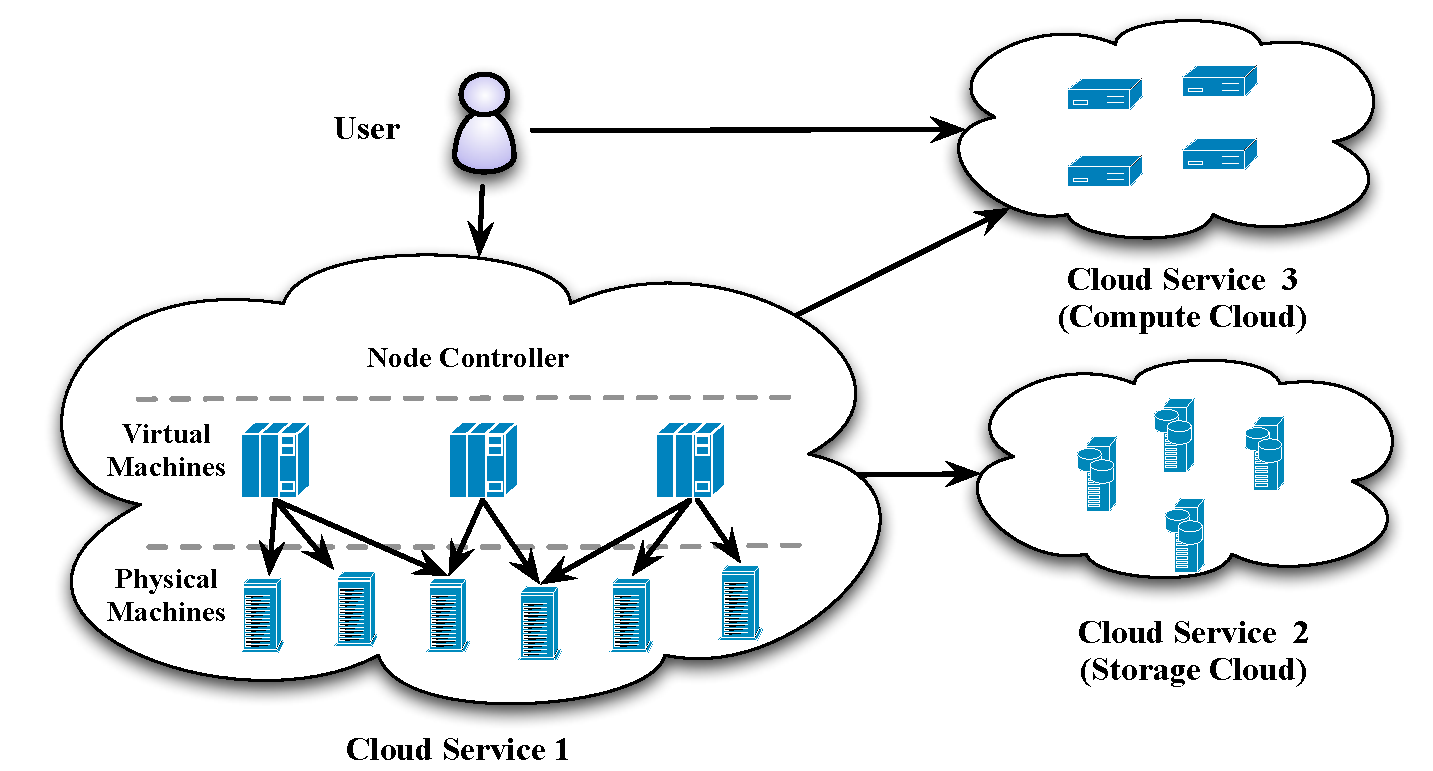
\includegraphics[width=14cm]{cloud-infra}
% where an .eps filename suffix will be assumed under latex, 
% and a .pdf suffix will be assumed for pdflatex; or what has been declared
% via \DeclareGraphicsExtensions.
\caption{A distributed cloud infrastructure consisting of multiple cloud services and virtualization.}
\label{fig:cloud-infra}
\end{figure*}



\subsection{Challenges and Features}
A distributed cloud environment presents a unique set of challenges for the development of a framework that will enable usage management of data that are stored, routed and processed by different services operating within the cloud environment. Figure~\ref{fig:cloud-infra} shows the layout of a typical cloud computing environment. A distributed cloud environment may consist of one or more cloud services that are owned by different entities. Services are often composable, and available to users or other services via web-services technologies such as REST and SOAP.  The services provide virtualized resources to cloud users that are provisioned on demand to meet the SLA terms that are negotiated between the cloud provider and the user. Within a cloud service implementation, the set of virtual resources are mapped onto a distributed infrastructure of physical resources as shown in Figure~\ref{fig:cloud-infra}. The desired features of a usage management framework for clouds, discussed below, are based on this generalized layout of distributed cloud systems.

\subsubsection {An open interoperable framework}

In order to enable data from different cloud users to move seamlessly across different service providers, and leverage the use of existing security mechanisms, it is necessary to design an open usage management framework. The framework must provide a scaffolding upon which different technologies can be built, that can interoperate via standardized interfaces. In order to achieve this, it is necessary to identify focal points within the framework that need to standardized, and areas that should {\em not} be standardized to enable differentiation and innovation~\cite{BlCl:01}. 

In order for the usage policies to be consistently interpreted across different cloud providers, it is necessary to develop a common, extensible cloud ontology. All usage policies need to be developed using such a common cloud ontology.  There have been efforts towards the development of such an ontology, although not for the purpose of usage policy specification~\cite{YuBuDa:08}. 

Different cloud services will have different requirements as far as policy language characteristics are concerned. These characteristics  include expressive power, reasoning power, and ease of use. Development of  a single standard policy language that intends to satisfy all these requirements will be bloated, and difficult to formalize and reason over. Moreover agreement on a standard policy language will stifle innovation, and such a  language may be unable to address the needs of  future cloud systems. Hence the framework must accommodate coexistence of multiple languages that interoperate, and allow seamless movement of data within the cloud. However, existence of multiple policy languages have lead to serious problems with interoperability and user satisfaction in other fields such as DRM~\cite{JaHeMa:06}. To prevent this, rather than having each service provider understand every other policy language, policy interpretation, validation and reasoning need to be carried out via standard interfaces and a common ontology agreed upon by all cloud providers. Existing policy management frameworks for distributed systems can be used to address these concerns~\cite{JaHeLa:10,DaDuLuSl:01}. This approach, explained in the next section, will provide enough room for the existence of multiple languages, and will allow for incorporation of new languages. 

Figure~\ref{fig:sla-usage} shows how usage management needs to incorporated in existing SLA frameworks and resource allocation mechanisms. At every level in a cloud infrastructure where resource allocation takes place, the resource allocation process is over-ridden by data usage policy. This means, prior to allocation of resources,  resource allocation controllers must consult usage policies associated with the data for which resources are being allocated. 


%An open framework for usage management must leverage  existing  SLA frameworks. Figure~\ref{fig:sla-usage} shows how such a framework could work along with existing SLA frameworks. In cloud environments, resource allocation occurs according to the terms of agreement in SLAs. For example, consider a cloud with an SLA that guarantees a given amount of compute time per compute batch. In such a scenario, if the size of the batch increases, the resource allocator will allocate more nodes for the batch. Hence the resource allocation control allocates resources in accordance with QoS parameters. As shown in Figure~\ref{fig:sla-usage} , usage management mechanism need to work along with this mechanism in order to ensure that the resource allocation is taking place according to the usage policy specified by the user. For example, the usage policy might prevent processing of the batch over clusters that fail to meet security requirements, owned by a particular company, or  located in a particular country. In such a scenario, the resource allocator will consult the usage policy before allocation of resources. 





\subsubsection{Dynamic interpretation}
Cloud computing services typically support a high degree of virtualization and dynamic composition of services. These two features have a different type of influence with respect to enforcement of QoS metrics and usage policy metrics. In the case of QoS metrics, enforcing the terms of the SLA agreement is solely the responsibility of the original cloud provider with whom the SLA is negotiated. Any other cloud services, engaged by the original cloud service provider to accomplish the task, have no responsibility towards respecting the original terms of agreement. In other words, QoS-based SLAs are brokered on a one-on-one basis, and have no bearing along the chain of servicing. 

On the other hand, usage policies need to be enforced by all service providers along the service chain that are a part of accomplishing the original task. For example if the original agreement mandates that the data cannot be stored in country $X$, then every cloud service along the chain which handles the data, must be capable of interpreting and enforcing this restriction. 

A cloud computing usage management framework must support dynamic interpretation of usage policies in order to enable usage policy enforcement across  service compositions and service chains. Dynamic interpretation allows policies to be expressed at a sufficient level of abstraction, and then interpreted appropriately depending on the particulars of a given cloud service environment~\cite{JaHeLa:10}. This ensures that usage policies are appropriately interpreted even if cloud users' data are passed on to cloud services with environments that are not known {\it a priori}. 

Another advantage of dynamic interpretation is that it takes into account the changes that occur within a given cloud service environment. This means that interpretation of a policy changes according to the changes that takes place in the cloud environment. For example, if the trusted computing base of a cloud service provider is attacked and becomes vulnerable, it allows the usage policies to be interpreted in a more strict manner after the attack. 

\begin{figure}[t]
\centering
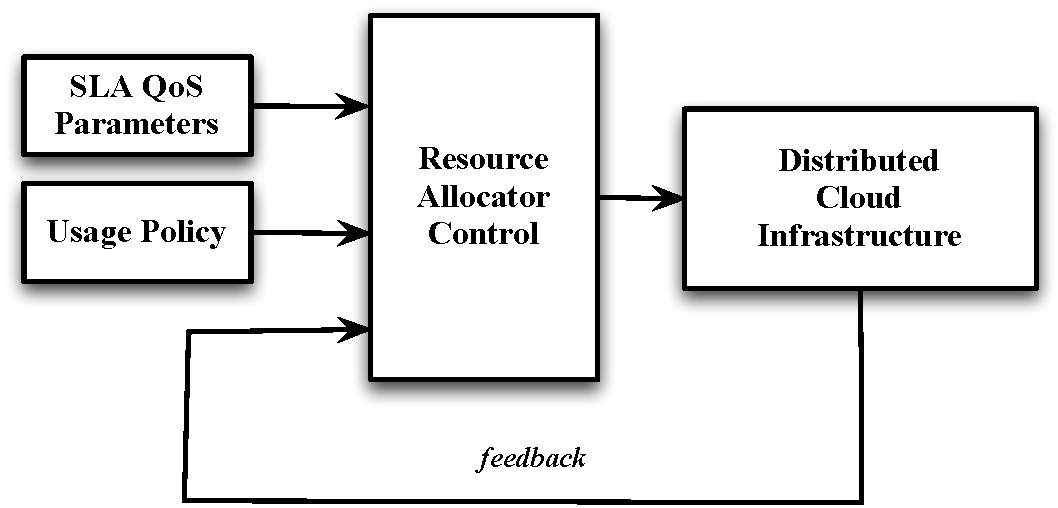
\includegraphics[width=9cm]{sla-usage}
%) where an .eps filename suffix will be assumed under latex, 
% and a .pdf suffix will be assumed for pdflatex; or what has been declared
% via \DeclareGraphicsExtensions.
\caption{Cloud usage management operating with SLA QoS monitoring.}
\label{fig:sla-usage}
\end{figure}



\subsubsection {Persistence}
In a cloud environment, data from multiple users may be handled by multiple cloud providers, and fractions of data sets may be stored, processed and routed across a geographically distributed computing infrastructure. Data are often subject to different types of transformations, aggregations and separations.  In such scenarios, it is necessary that all elements of a particular data set, associated with a given usage policy, are handled throughout their lifetime in the cloud, by different cloud services, in a manner that is consistent with the usage policy over the original data set. 

Usage management persistent across data aggregations is shown in Figure~\ref{fig:dynamics}. The service provided by Cloud Provider 1 aggregates multiple data form different sources, and feeds them to a service provided by Cloud Provider 2. In this scenario, each of the original data sources are governed by their own usage policies. After they are combined, the aggregated data set is governed by a combined usage policy that is a logical combination of the original two usage policies. Existing policy languages that support these combinations of policies may be used for this purpose~\cite{JaHe:08a}.

Enabling persistence in usage control requires the use of sophisticated naming, resolutions and policy manipulation mechanisms. It is necessary that in such scenarios, as data sets undergo transformations such as aggregation or separation, corresponding identifiers are created for the new data set, policies for the new data set are generated, and the new policies are attached to the corresponding data set. The policies may either by physically attached to the data set by means of encodings, or they may be attached via indirection. 


%As an example, consider Dataset 1 that is governed by Policy 1 which states: {\em ``This data set can only be stored in North America''}, and Dataset 2 which is governed by a Policy 2 which states: {\em ``This data set can only be stored in USA and Europe''}. After Dataset 1 and Dataset 2 are aggregated, the combined data set is governed by the logical combination of the two policies which states: {\em The aggregated data set can be stored only in USA''}. 

%In order to achieve this capability, it is necessary that underlying policy language support logical combination of policies, and reasoning over such operations. Additionally, the usage management framework must employ mechanisms that allow dynamic generation There exist usage policy languages that support such operations~\cite{JaHe:08}. 


\begin{figure}[!t]
\centering
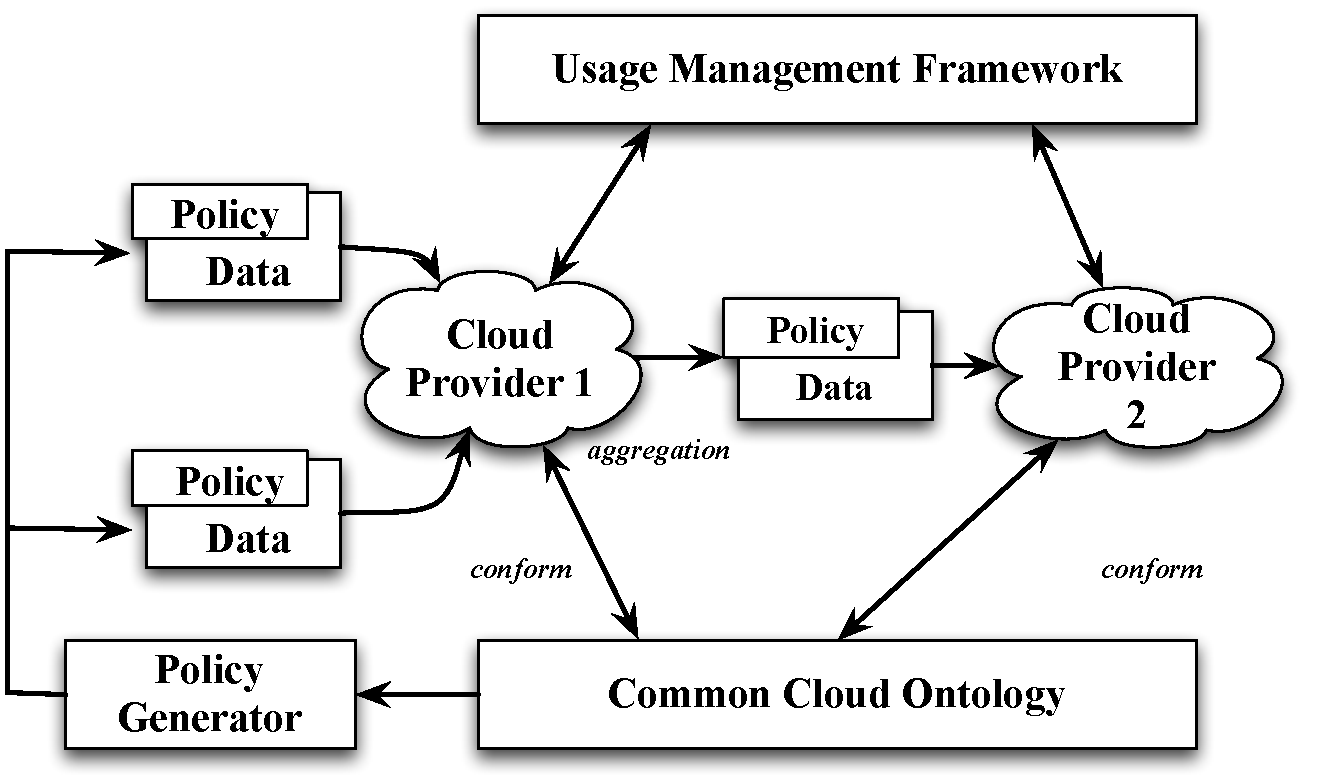
\includegraphics[scale=0.4]{dynamics}
% where an .eps filename suffix will be assumed under latex, 
% and a .pdf suffix will be assumed for pdflatex; or what has been declared
% via \DeclareGraphicsExtensions.
\caption{Persistence of policies across data aggregations.}
\label{fig:dynamics}
\end{figure}

\subsubsection{Policy and cloud infrastructure interconnection}
It is important that usage management mechanism in cloud computing allows to reason about usage policies with respect to the capabilities of the underlying cloud infrastructure. It must be possible for a cloud provider to determine in an automated manner what aspects of a usage policy can and cannot be enforced, the reasons for not being able to enforce a particular usage policy, and the overhead cost involved in enforcing a usage policy. These questions can answered in an automated manner only if policies are expressed in a formal way that can be reasoned over. 

The usage management framework must also enable service providers to leverage existing security services such as encryption mechanisms, trusted computing base, authentication mechanisms, naming and resolution mechanisms, trust management mechanisms, negotiation frameworks and existing SLA frameworks to provide comprehensive security solutions in the cloud computing arena. The framework must provide hooks that enable use these mechanisms to enforce usage policies. 

In the next section a preliminary architecture that will form a platform upon which an open interoperable usage management framework for cloud computing can be built is proposed. The architecture enables use of multiple usage policy languages across different cloud providers while allowing interoperability among them. 





\section{Proposed Architecture}\label{sec:architecture}
In this section a preliminary architecture for usage management in cloud computing is described. The proposed architecture is based on the goals, principles and features discussed in the previous section. The architecture builds upon the previous work usage management in distributed environments~\cite{JaHeLa:10}.  The operation of the proposed architecture is divided into two phases, namely, a Setup phase and a Working phase. The Setup phase deals with the agreement on a usage policy and the setup of the cloud environment, and the Working phase deals with interpretation and enforcement of usage policies. The proposed architecture is currently being implemented in Ruby on Rails web application framework, and provides a web interface supporting functions for expression of policies, registration of policies, interpretation and evaluation of policies, among others. The details of the architecture are described below.

\subsection{Setup Phase}
The underlying principle driving the design of proposed architecture is that policies are evaluated within a context, and a context is separated form the syntax and semantics of policy languages. A usage policy consists of restrictions over usage expressed in terms of  context properties.  A context provides a formal representation of the cloud environment within which a policy is interpreted. A context formally represents the entities within the environment, the relations among the entities, properties of the cloud environment, and the current state of the environment. 

\begin{figure}[t]
\centering
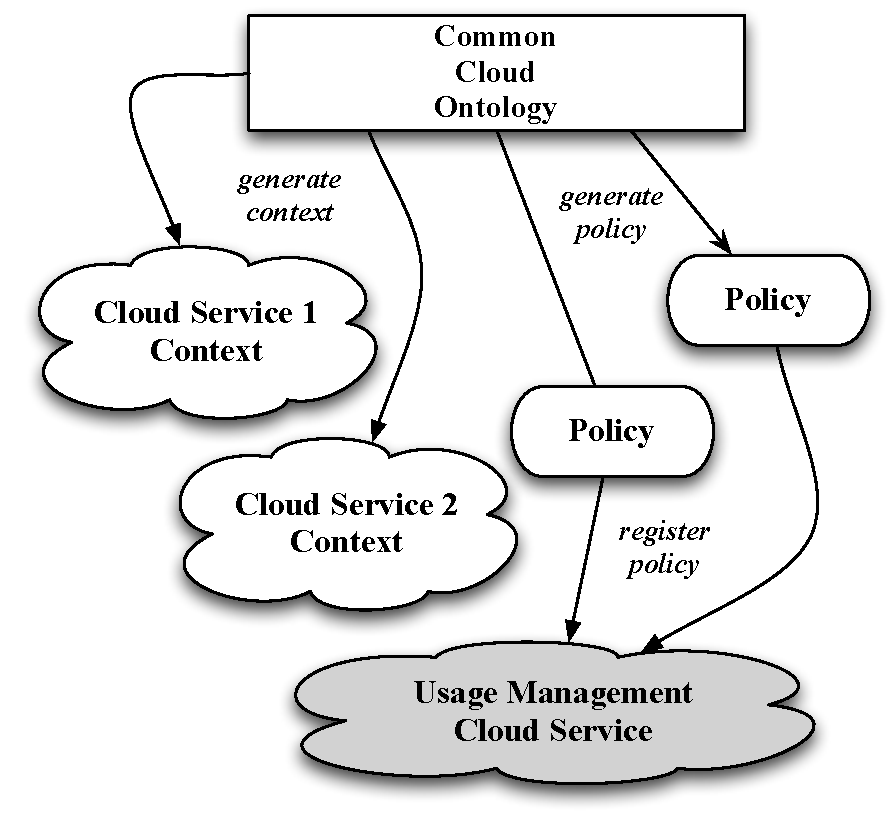
\includegraphics[width=9cm]{cloud-setup}
% where an .eps filename suffix will be assumed under latex, 
% and a .pdf suffix will be assumed for pdflatex; or what has been declared
% via \DeclareGraphicsExtensions.
\caption{Setup phase usage management that include context and license generation.}
\label{fig:cloud-setup}
\end{figure}

\begin{figure*}[!t]
\centering
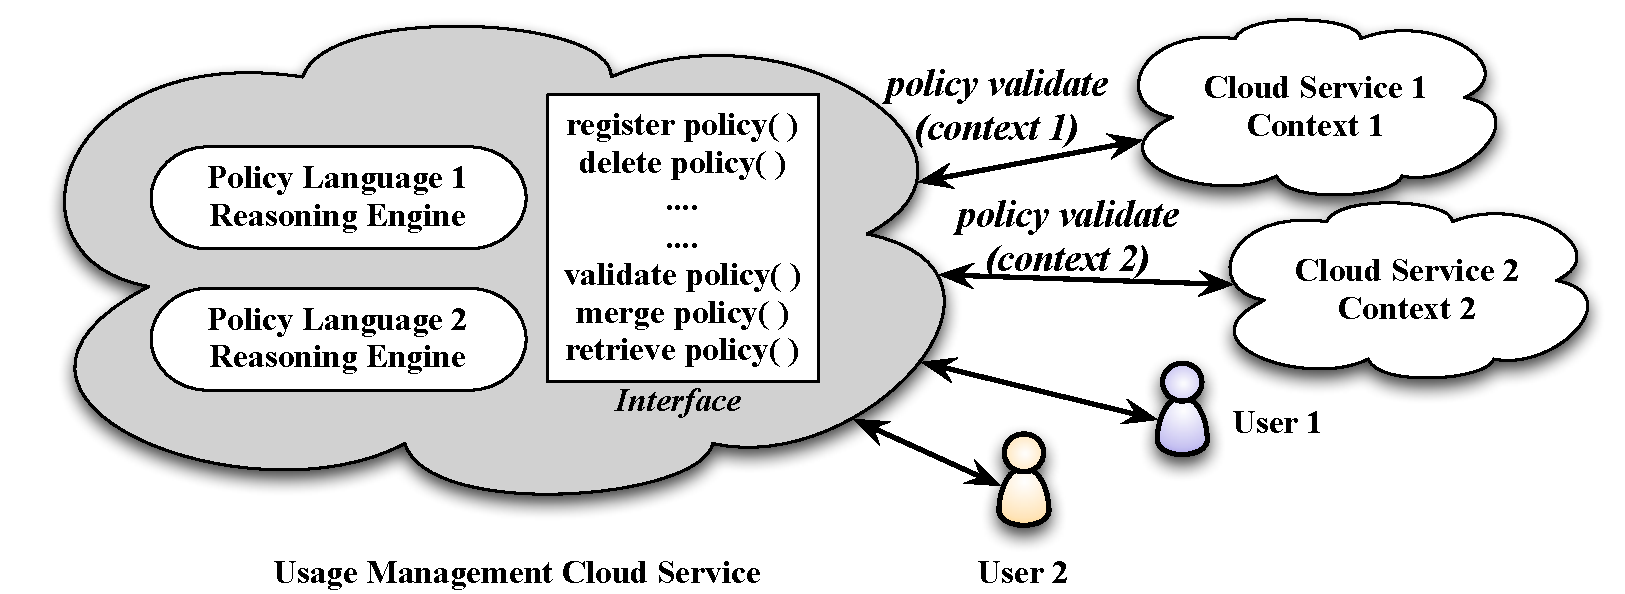
\includegraphics[width=13cm]{cloud-working}
% where an .eps filename suffix will be assumed under latex, 
% and a .pdf suffix will be assumed for pdflatex; or what has been declared
% via \DeclareGraphicsExtensions.
\caption{Operation of usage management in cloud environment.}
\label{fig:cloud-working}
\end{figure*}

As an example, consider a context for a cloud service consisting of  different data processing sub-services ({\em dps}). A simplified context may consist of the following parameters: $\{date, dps\_location, dps\_trust-level \}$, where $date$ represents the global date, $dps\_location$ represents the location of the sub-service, and $dps\_trust-level$ represents the trust level of the sub-service ranging form 1-5. Usage policies for the data are then expressed as restrictions over these parameters. For example, a rudimentary usage policy might state that {\em `` Data set X can be processed only by a $dps$ located in the USA, with trust levels greater than 4, and not beyond December 16th, 2013''. }

Even though the example presented above is oversimplified, the point to note is that every cloud service has a representative context whose state (values taken by the parameters in the context) is continually maintained with appropriate values. During the Setup phase, shown in Figure~\ref{fig:cloud-setup}, cloud services define and generate their own context from a common cloud ontology that is shared among all cloud services. Depending the type and nature of cloud services, services will share certain common context parameters such as time, date and location, whereas differentiate in terms of other parameters. Usage policies over users' data set are generated using the common cloud ontology. It can be seen that all the parameters, using which policy restrictions are described, must be well-defined in the context of the cloud environment within which the policy is to interpreted.

In the proposed architecture, the policy languages used for expressing the policies are not standardized. Different cloud services may use their choice policy languages depending on their expression and reasoning requirements. However, in order for policies to be interpreted across different cloud environments, it is necessary that all policies make use the terms defined in the common cloud ontology that is shared by all cloud services. The manner in which policies are interpreted in the operational phase is explained next. 



\subsection{Working Phase}
The Working phase consists of policy management, policy interpretation and validation via a common usage management cloud service that is shared by different services within the cloud. The operation of usage management cloud service is shown in Figure~\ref{fig:cloud-working}. Instead of standardizing a common policy language for all cloud services, in the proposed architecture, the usage management cloud service provides a standard web interface for managing policies. This standard interface allows policies to be registered, retrieved, attached to data sets, deleted, validated, interpreted, reasoned, and merged with other policies by different cloud services via an extensible web interface. 

In the proposed system, usage policies are validated by cloud services in the following manner. Cloud services query the usage management service for a particular action on a particular data set by providing the context under which the action is intended to be carried out. The usage management service then evaluates whether the policy and the context are interoperable by comparing the terms. If the terms are consistent, then the policy restrictions are evaluated with respect to the current state of the context provided. If the restrictions are satisfied, the action is given a go ahead, otherwise it is denied. Every policy maintains a state or history of the usage performed by different cloud services on the data set. Such a history is commonly maintained in usage control and DRM languages to enforce count limits or obligation semantics on certain actions over a data set. Data usage histories can also be potentially used to validate data use with respect to policy terms, and provide cloud users with usage tracking services for their data.

Cloud services can register policies expressed in different policy languages,  however, all the policies are queried by means of a standard web interface. This approach ensures that the syntax and semantics of different policy languages is hidden from the cloud services that need to query usage policies. This precludes the need for every cloud service provider to deploy an interpreter for different policy languages. In addition, a service provider can introduce a new policy language for its operations, along side its previous policies expressed in the old policy language in a seamless manner. Figure~\ref{fig:cloud-working} shows how multiple policy languages can operate behind a common, standardized web interface for usage policy management.

\section{Conclusions and Future Work}\label{sec:conclusions}
In this paper we introduced the notion of usage management in cloud computing environment. Cloud computing exhibits a unique set of characteristics that require usage management of users' data according to user concerns and expectations. We analyzed the challenges involved in the design and development of a framework for usage management in cloud environments. We showed that such a framework needs to be open to leverage existing security technologies and SLA frameworks. The framework needs to exhibit features such as support for multiple policy languages, existence of a common cloud ontology, dynamic interpretation and persistence of usage enforcement. Finally a preliminary framework that supports multiple policy languages was introduced that provides a platform upon which such a framework can be built. 

Future work involves efforts towards the development of a common extensible cloud ontology that will provide a common vocabulary for cloud environments and enable interoperability. Such an ontology needs be developed by taking into consideration the requirements of different cloud services. In addition, it is necessary to standardize interfaces for other security mechanisms mentioned in the paper that can be incorporated within the framework. Finally, existing policy languages can be modified to be incorporated within the framework, and new ones need to designed to address the specific needs of different cloud services. 


% An example of a floating figure using the graphicx package.
% Note that \label must occur AFTER (or within) \caption.
% For figures, \caption should occur after the \includegraphics.
% Note that IEEEtran v1.7 and later has special internal code that
% is designed to preserve the operation of \label within \caption
% even when the captionsoff option is in effect. However, because
% of issues like this, it may be the safest practice to put all your
% \label just after \caption rather than within \caption{}.
%
% Reminder: the "draftcls" or "draftclsnofoot", not "draft", class
% option should be used if it is desired that the figures are to be
% displayed while in draft mode.
%
%\begin{figure}[!t]
%\centering
%\includegraphics[width=2.5in]{myfigure}
% where an .eps filename suffix will be assumed under latex, 
% and a .pdf suffix will be assumed for pdflatex; or what has been declared
% via \DeclareGraphicsExtensions.
%\caption{Simulation Results}
%\label{fig_sim}
%\end{figure}

% Note that IEEE typically puts floats only at the top, even when this
% results in a large percentage of a column being occupied by floats.


% An example of a double column floating figure using two subfigures.
% (The subfig.sty package must be loaded for this to work.)
% The subfigure \label commands are set within each subfloat command, the
% \label for the overall figure must come after \caption.
% \hfil must be used as a separator to get equal spacing.
% The subfigure.sty package works much the same way, except \subfigure is
% used instead of \subfloat.
%
%\begin{figure*}[!t]
%\centerline{\subfloat[Case I]\includegraphics[width=2.5in]{subfigcase1}%
%\label{fig_first_case}}
%\hfil
%\subfloat[Case II]{\includegraphics[width=2.5in]{subfigcase2}%
%\label{fig_second_case}}}
%\caption{Simulation results}
%\label{fig_sim}
%\end{figure*}
%
% Note that often IEEE papers with subfigures do not employ subfigure
% captions (using the optional argument to \subfloat), but instead will
% reference/describe all of them (a), (b), etc., within the main caption.


% An example of a floating table. Note that, for IEEE style tables, the 
% \caption command should come BEFORE the table. Table text will default to
% \footnotesize as IEEE normally uses this smaller font for tables.
% The \label must come after \caption as always.
%
%\begin{table}[!t]
%% increase table row spacing, adjust to taste
%\renewcommand{\arraystretch}{1.3}
% if using array.sty, it might be a good idea to tweak the value of
% \extrarowheight as needed to properly center the text within the cells
%\caption{An Example of a Table}
%\label{table_example}
%\centering
%% Some packages, such as MDW tools, offer better commands for making tables
%% than the plain LaTeX2e tabular which is used here.
%\begin{tabular}{|c||c|}
%\hline
%One & Two\\
%\hline
%Three & Four\\
%\hline
%\end{tabular}
%\end{table}


% Note that IEEE does not put floats in the very first column - or typically
% anywhere on the first page for that matter. Also, in-text middle ("here")
% positioning is not used. Most IEEE journals/conferences use top floats
% exclusively. Note that, LaTeX2e, unlike IEEE journals/conferences, places
% footnotes above bottom floats. This can be corrected via the \fnbelowfloat
% command of the stfloats package.


% conference papers do not normally have an appendix


% use section* for acknowledgement


% trigger a \newpage just before the given reference
% number - used to balance the columns on the last page
% adjust value as needed - may need to be readjusted if
% the document is modified later
%\IEEEtriggeratref{8}
% The "triggered" command can be changed if desired:
%\IEEEtriggercmd{\enlargethispage{-5in}}

% references section
% can use a bibliography generated by BibTeX as a .bbl file
% BibTeX documentation can be easily obtained at:
% http://www.ctan.org/tex-archive/biblio/bibtex/contrib/doc/
% The IEEEtran BibTeX style support page is at:
% http://www.michaelshell.org/tex/ieeetran/bibtex/
\bibliographystyle{IEEEtran}
% argument is your BibTeX string definitions and bibliography database(s)
\bibliography{drm}
%
% <OR> manually copy in the resultant .bbl file
% set second argument of \begin to the number of references
% (used to reserve space for the reference number labels box)
%\begin{thebibliography}{1}

%\bibitem{IEEEhowto:kopka}
%H.~Kopka and P.~W. Daly, \emph{A Guide to \LaTeX}, 3rd~ed.\hskip 1em plus 0.5em minus 0.4em\relax Harlow, England: Addison-Wesley, 1999.

%\end{thebibliography}




% that's all folks
\end{document}


